\documentclass{article}
\usepackage[utf8]{inputenc}
\usepackage{graphicx}
\usepackage{french}
%
\includegraphics[width=6cm] {enseirb-matmeca.png}

\title{Projet S5 : Plan du rapport}
\author{ALOUANI THIVIN}
\date{December 2021}

\begin{document}
\maketitle

\tableofcontents
\newpage
\section{Introduction}
    {
    \subsection{Contexte}
    
    \subsection{Le sujet}
    
    
    \subsection{Problémtique}
    
    }




\newpage
\section{Approche}
    {
    
    \subsection{Outils utilisés et structuration des fichiers}
    {
    Lors de notre recherche de résolution du problème et de la conception du projet, nous avons utilisé plusieurs outils étudiés lors des cours du 1er semestre.
    
        \subsubsection{Git}
        {
        Pour la gestion de nos dépôts locaux et distants, nous avons opté pour le logiciel de gestion de versions décentralisé GIT, nous permettant une meilleure organisation pour la répartition des tâches.
        
        }
        
 
        \subsubsection{Emacs}
        {
        Nous avons utilisé l'éditeur de texte Emacs que nous avons étudié lors du cours d'Environnement de travail pour ses outils facilitant l'écriture du code.
        
        }
    
     
        \subsubsection{\LaTeX}
        {
        LaTeX permet une mise en page claire et une facilité d'écriture de documents scientifiques. Nous avons ainsi choisi de l'utiliser pour la rédaction de notre rapport.
        }
    
        \subsubsection{Makefile}
        {
        Un fichier Makefile est un fichier contenant un ensemble de directives utilisées par un outil d'automatisation (make). Ce fichier nous a permis de classer nos fichiers .c et .h de manière a effectuer nos compilations séparées sans nous soucier des dépendances entre nos différents fichiers
        
        }
    
    
    }
    \bigskip
    \subsection{Structuration des données}
        {
        \subsubsection{Structure world}
            {
            Nous avons implémenté notre monde sous la forme d'un tableau d'entiers où l'entier correspond à la couleur de la cellule. Nous avons de même implémenté les fonctions de création et d'affichage d'un monde.
            
            
           
            }
        \subsubsection{Structure rule}
            {
            Au cours du projet nous avons donné différentes implémentations des règles d'évolution des cellules, nous avions d'abord opté pour une liste chaînée de structures 'rule' avant de nous tourner vers un tableau de structures que nous trouvions plus simple d'utilisation. Nous avons également implémenté les fonctions de manipulation de nos structures.
        
           
            }
        \subsubsection{Structure queue}
            {
            Le sujet du projet nous demandait d'implémenter une structure de type first in first out, de même que pour les règles nous avons implémenté la file de 2 manières différentes, une première fois avec un tableau et une seconde fois avec une liste chaînée. Nous avons également implémenté les fonctions de manipulation de nos structures.
             
            }
    
    
    
        }
    
    
    
    
    
    }


\newpage
\section{Résultats}

    {
    
    \subsection{Baseline}
        {
        \subsubsection{Version de base et indéterminisme}
        {
        A l'aide de nos structures implémentées précédemment nous avons pu définir les règles présentées dans le début du projet. Nous avons également adapté notre structure de règle pour que chaque règle puisse aboutir à plusieurs couleurs différentes.
        
        }
    
        \subsubsection{Le jeu de la vie}
        {
        Nous avons adapté notre structure de règle afin d'implémenter le jeu de la vie, il nous paraissait en effet compliqué de définir une à une les règles étant donnée notre implémentation précédente.
        
        }
        
        
        \subsubsection{Mouvements et incompressibilité}
            {
            Nous avons du revoir notre structure de règle pour prendre en compte les déplacements des cellules. Nous avons par ailleurs ajouter un système de file afin de gérer les différents mouvements et par la suite les problèmes d'incompressibilité.
            
            }
    
        }
    
    
    
    
    \subsection{Tests}
        {
        \subsubsection{Première règle}
            {
            Nous avons mis en place des tests afin de vérifier le fonctionnement de notre code, ceux-ci sont constitués d'un main appelant nos fonctions afin de créer un monde aléatoire et appliquer à chacune de ses cellules les règles de la version de base avec et sans déterminisme.
        
        
        
            }
        
        
        \subsubsection{Jeu de la vie}
            {
            Nous avons créé un fichier main qui définit un monde de taille demandée et y applique les règles du jeu de la vie.
        
        
            }
        
        \subsubsection{Modélisations des mouvements d'un grain de sable}
            {
            
            Afin de tester nos fonctions d'implémentation du mouvement des cellules nous avons défini des règles modélisant la chute et l'entassement de grains de sable et les avons testé d'un main, le moodèle semble correct malgré quelques incohérences vis-à-vis de la réalité physique.
            
            }
        
        
        
        }
    
    }

\newpage
\section{Conclusion}

    {
    
    
    
    
    
    }
\newpage
\centering{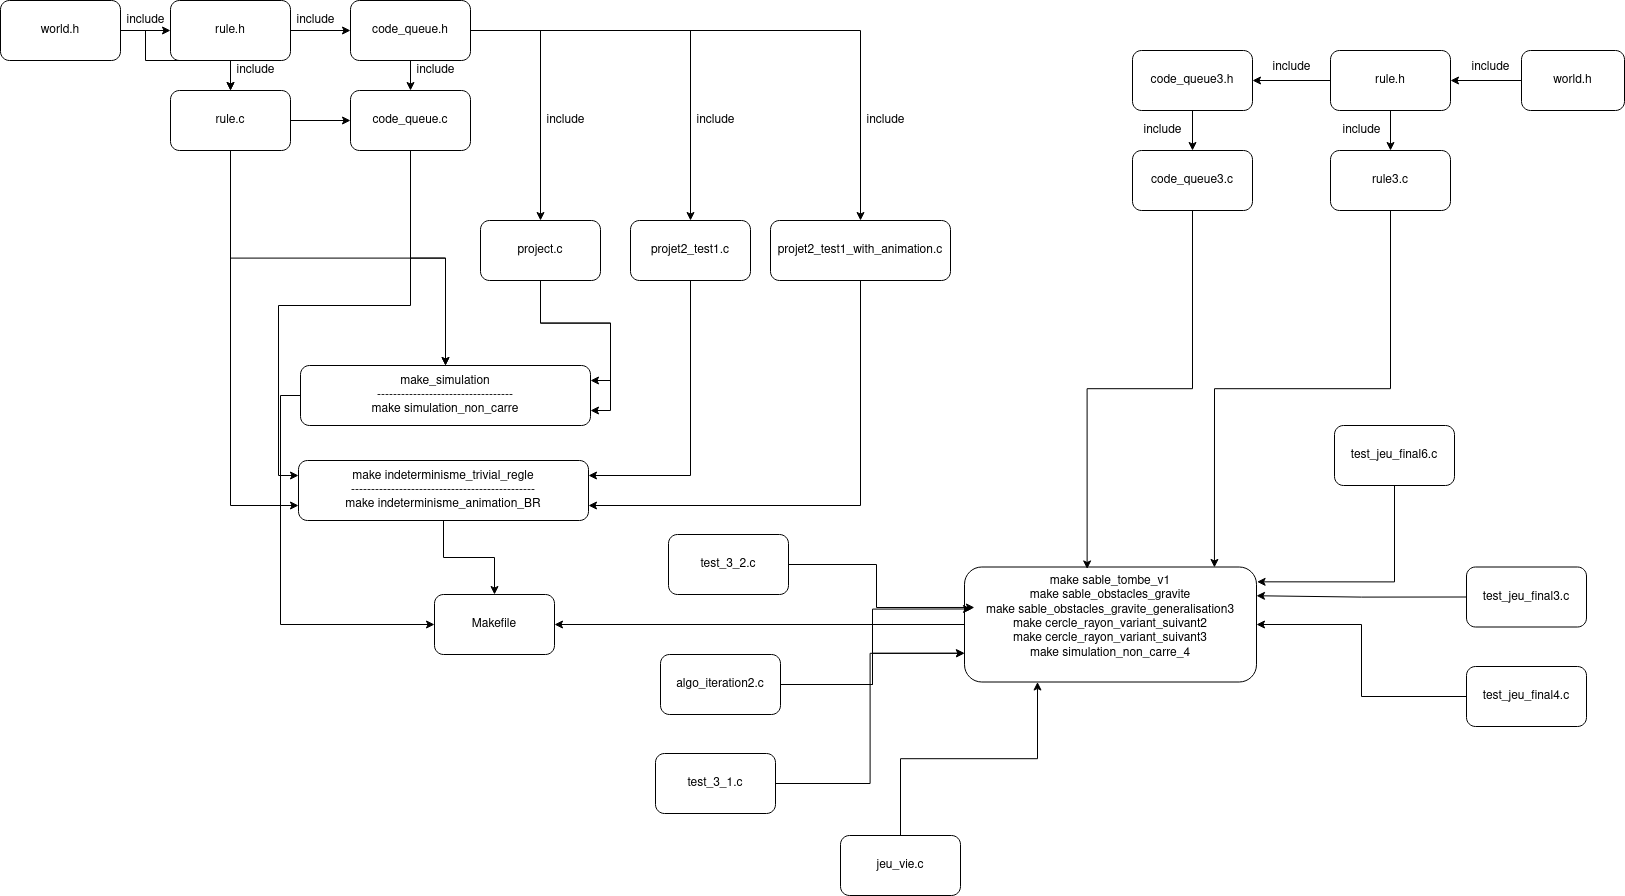
\includegraphics[scale=0.27] {graphe_des_dependances.png}}


\end{document}
